% Étape 8 : la tête, retour aux pixels (FreeFlow)
% Compiler avec pdflatex (ou Overleaf).
\documentclass[border=10pt]{standalone}
\usepackage[T1]{fontenc}
\usepackage[utf8]{inputenc}
\usepackage[scaled]{helvet}
\renewcommand{\familydefault}{\sfdefault}
\usepackage{sansmath}
\sansmath
\usepackage{amsmath}
\usepackage{tikz}
\usetikzlibrary{arrows.meta}

\definecolor{bleu}{HTML}{9CC8F0}    % Z : 1 carreau = 1 patch
\definecolor{vert}{HTML}{A8DCA0}    % 4096 canaux
\definecolor{rouge}{HTML}{F4A6A6}   % U, flot
\definecolor{jaune}{HTML}{FFE27A}   % confiance
\definecolor{gris}{HTML}{CCCCCC}
\definecolor{grisclair}{HTML}{F2F2F2}
\definecolor{noir}{HTML}{222222}

\tikzset{
  th/.style={font=\fontsize{14}{16}\selectfont\bfseries, text=black, inner sep=0pt},
  ts/.style={font=\fontsize{12}{14}\selectfont, text=black, inner sep=0pt},
  tm/.style={font=\fontsize{13}{15}\selectfont, text=black, inner sep=0pt},
  fl/.style={noir, line width=1.5pt, -{Stealth[length=7pt]}},
}
\newcommand{\num}[1]{\tikz[baseline=(c.base)]\node[circle,draw=black,line width=0.7pt,inner sep=1pt,font=\fontsize{10}{10}\selectfont\bfseries](c){#1};}
\newcommand{\grid}[6]{%
  \fill[#6] (#1,#2) rectangle ++(#4*#5,#3*#5);
  \ifnum#4>1 \foreach \k in {1,...,\numexpr#4-1\relax} \draw[white, line width=0.8pt] (#1+\k*#5,#2) -- ++(0,#3*#5); \fi
  \ifnum#3>1 \foreach \k in {1,...,\numexpr#3-1\relax} \draw[white, line width=0.8pt] (#1,#2+\k*#5) -- ++(#4*#5,0); \fi}

\begin{document}
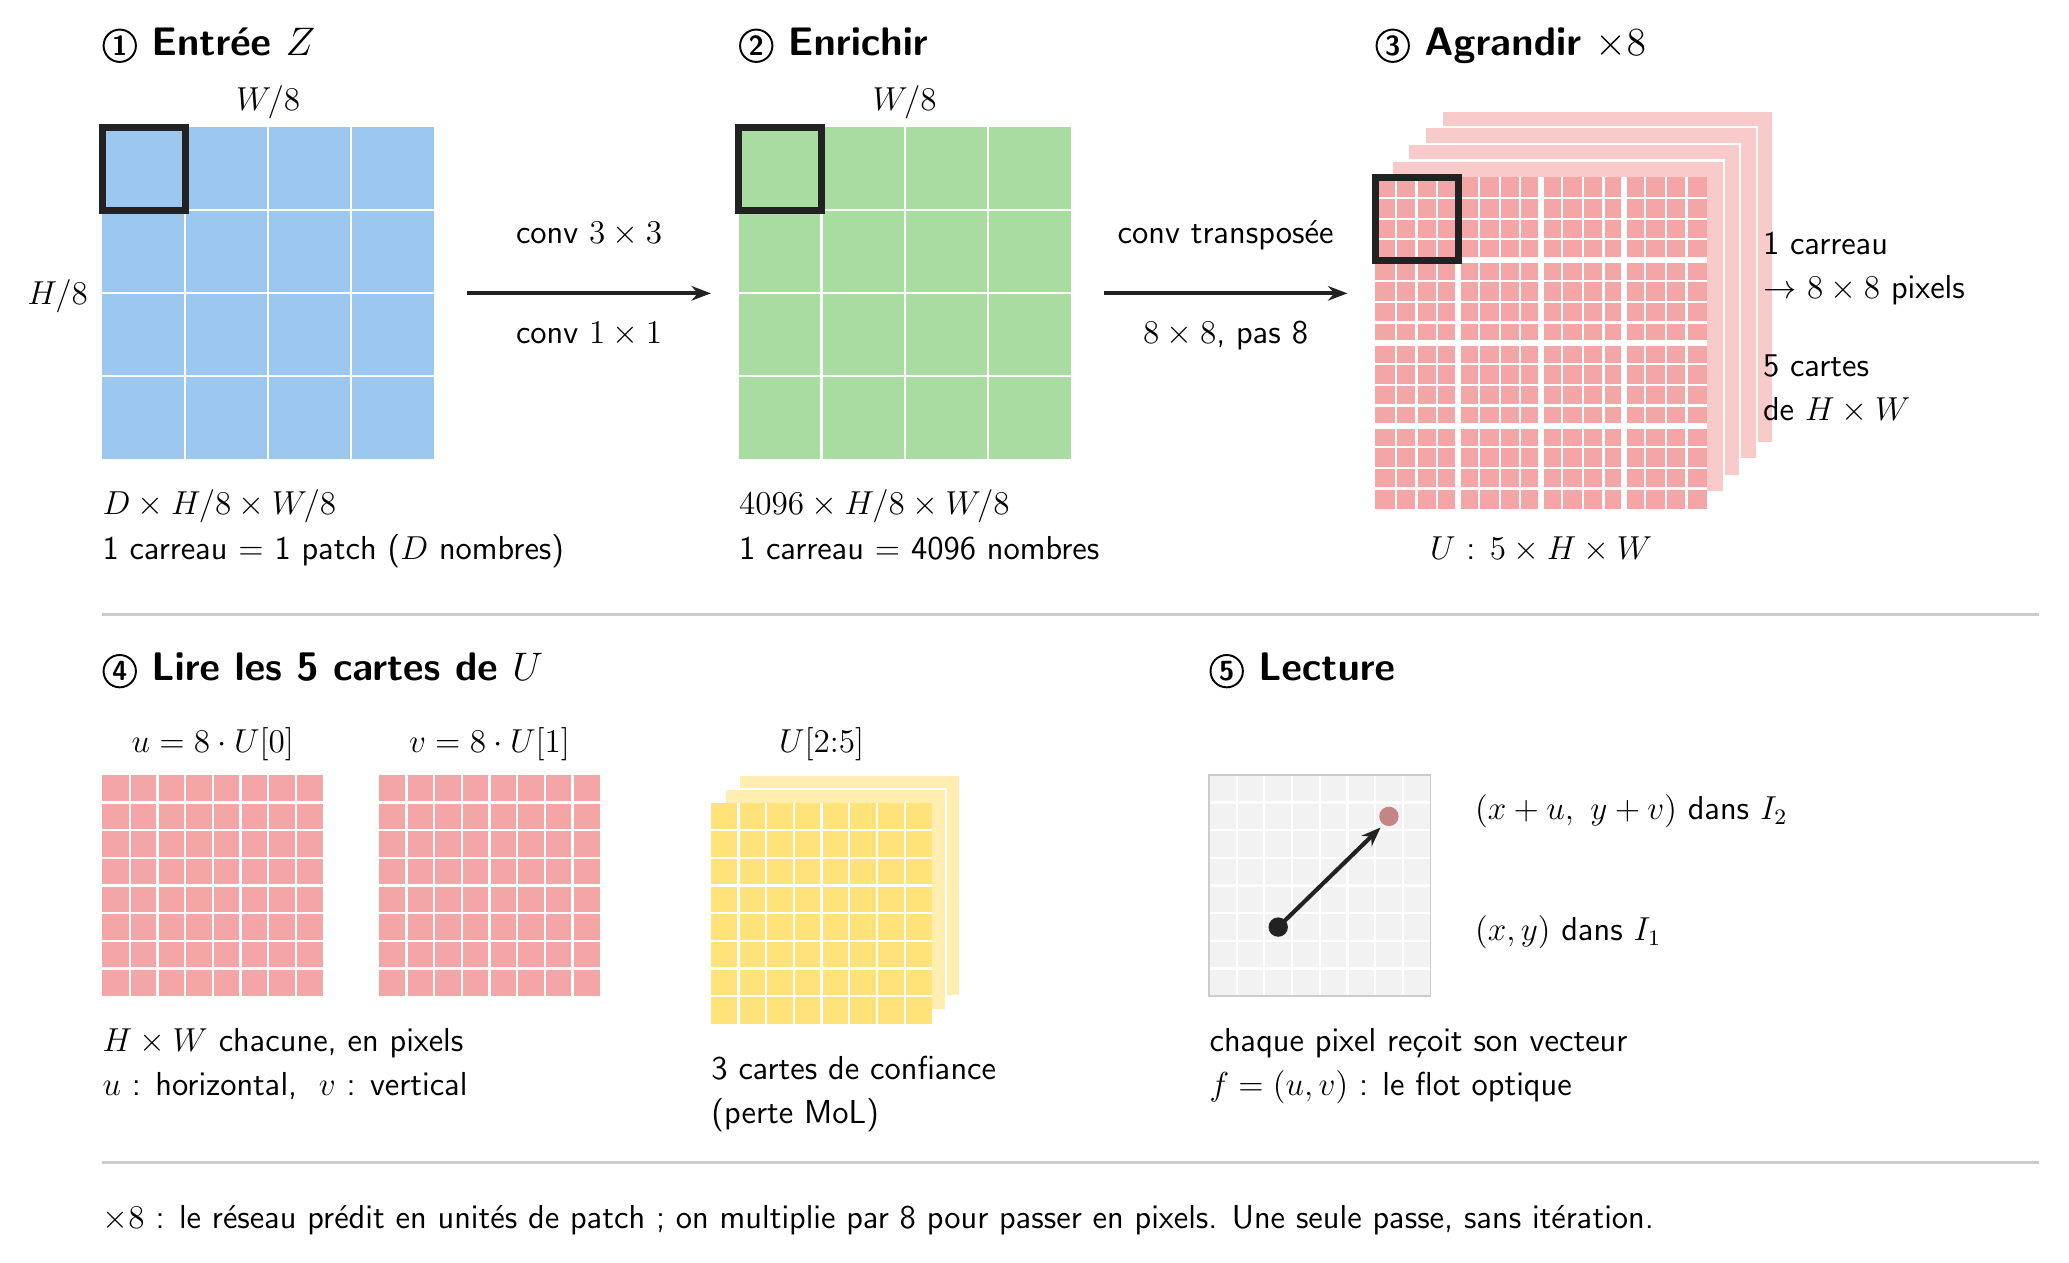
\begin{tikzpicture}[x=1pt, y=-1pt, line join=miter]

% =============== LIGNE 1 ===============
\node[th, anchor=base west] at (40,24)  {\num{1} Entrée $Z$};
\node[th, anchor=base west] at (270,24) {\num{2} Enrichir};
\node[th, anchor=base west] at (500,24) {\num{3} Agrandir $\times 8$};

% 1. Z en grille
\grid{40}{50}{4}{4}{30}{bleu}
\draw[noir, line width=2.5pt] (40,50) rectangle ++(30,30);
\node[ts, anchor=base] at (100,44) {$W/8$};
\node[ts, anchor=base] at (24,114) {$H/8$};
\node[ts, anchor=base west] at (40,190) {$D \times H/8 \times W/8$};
\node[ts, anchor=base west] at (40,206) {1 carreau = 1 patch ($D$ nombres)};

\draw[fl] (172,110) -- (260,110);
\node[ts, anchor=base] at (216,92) {conv $3 \times 3$};
\node[ts, anchor=base] at (216,128) {conv $1 \times 1$};

% 2. 4096 canaux par carreau
\grid{270}{50}{4}{4}{30}{vert}
\draw[noir, line width=2.5pt] (270,50) rectangle ++(30,30);
\node[ts, anchor=base] at (330,44) {$W/8$};
\node[ts, anchor=base west] at (270,190) {$4096 \times H/8 \times W/8$};
\node[ts, anchor=base west] at (270,206) {1 carreau = 4096 nombres};

\draw[fl] (402,110) -- (490,110);
\node[ts, anchor=base] at (446,92) {conv transposée};
\node[ts, anchor=base] at (446,128) {$8 \times 8$, pas 8};

% 3. U : 5 cartes H x W
\foreach \k in {4,3,2,1}
  \filldraw[fill=rouge!60, draw=white, line width=0.8pt] (500+6*\k,50+18-6*\k) rectangle ++(120,120);
\grid{500}{68}{16}{16}{7.5}{rouge}
\foreach \k in {1,2,3} {
  \draw[white, line width=2pt] (500+30*\k,68) -- ++(0,120);
  \draw[white, line width=2pt] (500,68+30*\k) -- ++(120,0);
}
\draw[noir, line width=2.5pt] (500,68) rectangle ++(30,30);
\node[ts, anchor=base] at (560,206) {$U$ : $5 \times H \times W$};
\node[ts, anchor=base west] at (640,96)  {1 carreau};
\node[ts, anchor=base west] at (640,112) {$\rightarrow$ $8 \times 8$ pixels};
\node[ts, anchor=base west] at (640,140) {5 cartes};
\node[ts, anchor=base west] at (640,156) {de $H \times W$};

% =============== LIGNE 2 ===============
\draw[gris, line width=1pt] (40,226) -- (740,226);
\node[th, anchor=base west] at (40,250) {\num{4} Lire les 5 cartes de $U$};

\node[tm, anchor=base] at (80,276) {$u = 8 \cdot U[0]$};
\grid{40}{284}{8}{8}{10}{rouge}
\node[tm, anchor=base] at (180,276) {$v = 8 \cdot U[1]$};
\grid{140}{284}{8}{8}{10}{rouge}
\node[ts, anchor=base west] at (40,384) {$H \times W$ chacune, en pixels};
\node[ts, anchor=base west] at (40,400) {$u$ : horizontal, \ $v$ : vertical};

\node[tm, anchor=base] at (300,276) {$U[2{:}5]$};
\foreach \k in {2,1}
  \filldraw[fill=jaune!60, draw=white, line width=0.8pt] (260+5*\k,294-5*\k) rectangle ++(80,80);
\grid{260}{294}{8}{8}{10}{jaune}
\node[ts, anchor=base west] at (260,394) {3 cartes de confiance};
\node[ts, anchor=base west] at (260,410) {(perte MoL)};

% =============== 5. Lecture ===============
\node[th, anchor=base west] at (440,250) {\num{5} Lecture};
\grid{440}{284}{8}{8}{10}{grisclair}
\draw[gris, line width=0.6pt] (440,284) rectangle ++(80,80);
\fill[noir] (465,339) circle (3.5);
\draw[fl] (465,339) -- (502,303);
\fill[rouge!80!black] (505,299) circle (3.5);
\node[ts, anchor=base west] at (536,300) {$(x + u,\ y + v)$ dans $I_2$};
\node[ts, anchor=base west] at (536,344) {$(x, y)$ dans $I_1$};
\node[ts, anchor=base west] at (440,384) {chaque pixel reçoit son vecteur};
\node[ts, anchor=base west] at (440,400) {$f = (u, v)$ : le flot optique};

\draw[gris, line width=1pt] (40,424) -- (740,424);
\node[tm, anchor=base west] at (40,448) {$\times 8$ : le réseau prédit en unités de patch ; on multiplie par 8 pour passer en pixels. Une seule passe, sans itération.};

\end{tikzpicture}
\end{document}
